\chapter{Support Vector Machines}
Precedentemente abbiamo introdotto:
\begin{itemize}
    \item \textbf{Percettrone semplice}: è un algoritmo di apprendimento efficiente
          solo per funzioni di separazione lineare.
    \item \textbf{Percettrone multistrato}: è un algoritmo difficile da addestrare
          perché deve aggiornare molti pesi e ci sono molti minimi locali, apprende
          sia funzioni lineari che non lineari.
\end{itemize}
Le \textbf{Support Vector Machines} (SVM) sono un algoritmo efficiente per
apprendere funzioni di separazione non lineari complesse.

Anche nel caso delle SVM viene ripreso comunque il concetto di separazione lineare,
ma con una scelta dell'iperpiano migliore. Si usa la \textit{teoria statistica
    dell'apprendimento}, utilizzando la \textbf{programmazione matematica}, la quale
dice che tra tutti gli iperpiani che possiamo usare per separare due classi, si
sceglie quello che sia in grado di etichettare meglio nel futuro. L'intuizione
è quella di prendere un iperpiano ottimo rispetto alla misura della distanza minima
che si ha tra gli esempi. Si guardano quindi tutti i punti del training set e
cerco di piazzare in mezzo l'iperpiano, in modo che intorno ad esso ci sia massima
ampiezza. Tale ampiezza è detta \textbf{margine}.
\begin{definizione}[\textbf{Margine}]
    Il margine è la distanza tra i vettori di supporto e l'iperpiano.
\end{definizione}
Se riuscissimo a separare i dati con un largo margine avremmo ragione di credere
che il classificatore sia “più robusto” tanto da avere una migliore generalizzazione.
Quando arriva quindi un nuovo punto, generato con la stessa regola degli altri,
sarà più probabilmente classificato in modo corretto, una volta scelto l'iperpiano.

Ci serve quindi la separabilità delle istanze, serve quindi che la funzione generatrice
sia linearmente separabile.
\begin{teorema}[\textbf{Dimensione di Vapnik-Cervonenkis}]
    Con la teoria statistica dell'apprendimento si dimostra che più allarghiamo
    il margine meglio l'iperpiano generalizza, raggiungendo la dimensione di
    Vapnik-Cervonenkis (VC). Prese tutte le funzioni che generano il training
    set si produce la Vapnik-Cervonenkis che esprime quanto è difficile sbagliare
    sulle ipotesi future in base alla scelta dell'iperpiano.
\end{teorema}
Dobbiamo quindi scrivere un algoritmo per trovare l'iperpiano di separazione di
massimo margine. In input si hanno le istanze etichettate e in output un vettore
che identifica l'iperpiano. Viene usata una notazione matematica, la quale prevede
che, preso un insieme di punti di training:
\begin{equation}
    S = \{(x_1, y_1), (x_2, y_2),\dots, (x_n, y_n)\}
\end{equation}
dove ad ogni vettore $x_i$ associo la classe di appartenenza $y_i$:
\begin{equation}
    y_i \in \{-1, +1\}
\end{equation}
ho i punti linearmente separabili nel seguente modo:
\begin{equation}
    \begin{cases}
        \langle w, x_i \rangle + b > 0 & \text{se} \ y_i = +1 \\
        \langle w, x_i \rangle + b < 0 & \text{se} \ y_i = -1
    \end{cases}
\end{equation}
questo può essere riassunto in un solo vincolo nel seguente modo:
\begin{equation}
    y_i(\langle w, x_i\rangle + b) > 0, \  i = 1,\dots, n
\end{equation}
Si ha che il vettore $w$ mi dirà l'inclinazione del piano mentre $b$ è la distanza
tra l'origine e il piano, queste due variabili identificano i vari iperpiani
possibili tra cui cercare il migliore.

L'ipotesi quindi tra $w$ e $b$ è una funzione che prende il segno di $\langle w,
    x \rangle + b$ per associare l'etichetta:
\begin{equation}
    h_{w,b} (x) = sgn(\langle w, x \rangle + b)
\end{equation}
Siano $d_{-}$ e $d_{+}$ le distanze tra l'iperpiano separatore e il punto positivo
e negativo più vicino, allora definiamo:
\begin{itemize}
    \item \textbf{Margine funzionale}.
    \item \textbf{Margine geometrico}.
\end{itemize}
\begin{definizione}[\textbf{Margine funzionale}]
    Definiamo il \textbf{margine funzionale} di un punto $(x_i, y_i)$ rispetto
    all'iperpiano $(w, b)$ come:
    \begin{equation}
        \hat{\gamma}_i = y_i( \langle w, x_i \rangle + b )
    \end{equation}
    e quindi il margine funzionale dell'iperpiano rispetto al training set $S$ è
    definito come:
    \begin{equation}
        \hat{\rho} = \min_{i = 1, \dots, n} \hat{\gamma}_i
    \end{equation}
\end{definizione}
Si hanno quindi due casistiche:
\begin{enumerate}
    \item Se si ha un punto $x_i$ tale che $y_i = +1$, perché il margine
          funzionale sia grande è necessario che la quantità $\langle w, x_i
              \rangle + b$ abbia un grande valore positivo.
    \item Se si ha un punto $x_i$ tale che $y_i = -1$, perché il margine funzionale
          sia grande è necessario che la quantità $\langle w, x_i \rangle + b$
          abbia un grande valore negativo.
\end{enumerate}
Il margine funzionale specifica quanto è buona la classificazione, ma non misura
la distanza degli esempi dall'iperpiano.
\begin{teorema}
    Se $\hat{\gamma}_i > 0$, per ogni $classificazione_i$ la classificazione è
    approvata in quanto le classi sono linearmente separabili e l'iperpiano
    $(w, b)$ separa effettivamente le classi
\end{teorema}
Si ha quindi che un ampio margine funzionale fornisce una maggior qualità
di previsione, anche, se l'uso del solo $\hat{\gamma}$ può essere problematico,
in quanto il margine funzionale non è invariante rispetto ad un iperpiano ri-scalato.

Per come è stato scelto il classificatore $f$, se si scala l'iperpiano:
\begin{equation}
    (w, b) \to (c \cdot w, c\cdot b)
\end{equation}
si ottengono:
\begin{itemize}
    \item Lo stesso iperpiano, ovvero lo stesso luogo di punti.
    \item La stessa funzione di decisione, visto che quest'ultima dipende solo
          dal segno di $\langle w, x \rangle + b$, con il segno che può essere
          invertito se $c < 0$.
\end{itemize}
ma dato che il margine funzionale viene moltiplicato per $c$, non possiamo usarlo
come distanza di un punto dall'iperpiano, perché non è \textbf{invariante} rispetto
alla scala. Bisogna studiare la distanza $d$ del punto $x$ dall'iperpiano. Si ha
quindi:
\begin{equation}
    d = \frac{\sum_{i = 1} ^ n w_i \cdot x_i + b}{\| w \|} =
    \frac{\langle w, x_i \rangle + b}{\|  w \|}
\end{equation}
\begin{definizione}[\textbf{Margine geometrico}]
    Definiamo il \textbf{margine geometrico} di un punto $(x_i, y_i)$ rispetto
    all'iperpiano $(w, b)$ come:
    \begin{equation}
        \gamma = \frac{y_i(\langle w, x_i \rangle + b)}{\| w \|}
    \end{equation}
    e quindi il margine geometrico dell'iperpiano rispetto al training set $S$ è
    definito come:
    \begin{equation}
        \rho =  \min_{i = 1, \dots, n} {\gamma}_i
    \end{equation}
\end{definizione}
A differenza del margine funzionale, quello geometrico ci specifica quanto
sono distanti i punti dall'iperpiano.
\begin{teorema}
    Se $\gamma_i > 0$, per ogni $classificazione_i$ la classificazione è approvata
    analogamente a quanto detto per il margine funzionale.
\end{teorema}
Dato un punto positivo/negativo il margine geometrico rappresenta la sua distanza
geometrica dall'iperpiano, rende meglio l'idea della distanza di un punto da un
iperpiano in $\mathbb{R}^n$.

Inoltre, si ha che è invariante rispetto alla scala di $w$ e quindi possiamo
scalare l'iperpiano senza cambiamenti della distanza dei punti rispetto
all'iperpiano, in questo modo il margine rimane invariato. Al contrario il
margine funzionale è variante perché cambiando la scala di $w$ allora cambiava
anche il valore del margine, cambiando la semantica della classificazione, ciò
comporta errori.

Dalla formula notiamo che, posto $\| w \| = 1$ si scala l'iperpiano $(w, b)$:
\begin{equation}
    (w, b) \to \left(\frac{w}{\|w\|}, \frac{b}{\| w\|}\right)
\end{equation}
Si considera quindi un iperpiano $\left(\frac{w}{\|w\|}, \frac{b}{\| w\|}\right)$
con il vettore di pesi $\frac{w}{\| w \|}$ di norma unitaria.
\begin{definizione}[\textbf{Iperpiano canonico}]
    Definiamo un \textbf{iperpiano canonico} se:
    \begin{equation}
        \min_{i = 1, \dots, n} |\langle w, x_i \rangle + b| =  1
    \end{equation}
    e quindi, per un iperpiano canonico si hanno:
    \begin{itemize}
        \item margine funzionale pari a $1$
        \item margine geometrico pari a $\frac{1}{\| w \|}$
    \end{itemize}
\end{definizione}
Si nota che se $\| w \| = 1$ allora margine funzionale e geometrico coincidono,
infatti si possono mettere in correlazione:
\begin{equation}
    \gamma = \frac{\hat{\gamma}}{\| w \|}
\end{equation}
Bisogna quindi cercare di estendere il margine, cerchiamo quindi di massimizzare
una certa funzione obiettivo:
\begin{equation*}
    \begin{aligned}
        \max f(x) \\ \text{s.t.} \ g(x) \leq 0 \\ h(x) = 0
    \end{aligned}
\end{equation*}
Vorremmo assicurarci che tutti i punti cadano al di fuori del margine
(\textbf{hard margin}) e quindi, dato un certo $\gamma$ vogliamo che $\forall i
    \in \{1, \dots, n\}$:
\begin{equation}
    \frac{y_i \cdot (\langle w, x_i \rangle + b)}{\| w \|} \geq \gamma
\end{equation}
e quindi vogliamo:
\begin{equation*}
    \begin{aligned}
        \max \gamma \\ \text{s.t.} \ y_i (\langle w, x_i \rangle + b) \geq
        \gamma      \\ \| w \| = 1
    \end{aligned}
\end{equation*}
vincolando il margine geometrico ad essere uguale a quello funzionale.
Riscriviamo quindi:
\begin{equation*}
    \begin{aligned}
        \max \frac{\hat{\gamma}}{\|w\|} \\ \text{s.t.} \ y_i(\langle w, x_i
        \rangle + b) \leq \gamma
    \end{aligned}
\end{equation*}
Non avendo comunque un vincolo convesso.

Possiamo però scalare l'iperpiano senza variazioni, grazie all'invarianza.
Lo scalo quindi in modo da avere l'iperpiano canonico, con margine funzionale
pari a 1:
\begin{equation*}
    \begin{aligned}
        \max \frac{1}{\|w\|} \\ \text{s.t.} \ y_i(\langle w, x_i \rangle + b)
        \leq \gamma
    \end{aligned}
\end{equation*}
Si cerca quindi di rendere massimo $\frac{1}{\|w\|}$ che equivale a rendere
minimo $\frac{1}{2} \| w \|^2$. Quindi si ottiene che vogliamo minimizzare
$\frac{1}{2} \| w \|^2$, che per comodità chiamiamo $\tau (w)$:
\begin{equation*}
    \begin{aligned}
        \min \tau(w) = \frac{1}{2}  \| w\|^2 \\ \text{s.t.} \ y_i (\langle w, x_i
        \rangle + b) \leq \gamma
    \end{aligned}
\end{equation*}
\begin{teorema}
    Si dimostra che esiste una sola soluzione al problema, ovvero esiste un unico
    iperpiano di massimo margine.
\end{teorema}
Ricapitolando si hanno due ragioni a supporto delle SVM:
\begin{enumerate}
    \item La generalizzazione, ovvero la capacità dell'iperpiano di separazione
          di massimo margine.
    \item Esiste un'unica soluzione del problema di ottimizzazione appena descritto.
\end{enumerate}
Si sta cercando:
\begin{equation*}
    \begin{aligned}
        \min \tau(w) = \frac{1}{2}  \| w\|^2 \\ \text{s.t.} \ y_i (\langle w, x_i
        \rangle + b) \leq \gamma
    \end{aligned}
\end{equation*}
e si ha che:
\begin{equation}
    w = \sum_{i \in Q} \alpha_i \cdot x_i
\end{equation}
ovvero scritta in termini di un sottoinsieme di esempi del training set che
giacciono sul margine dell'iperpiano, anche noto come \textbf{vettori di supporto},
prendendo una somma pesata dei contenuti dei vettori.

Il passaggio finale è che, se ho $\langle w, x \rangle + b$ che indicano cosa ho
appreso, se ricevo un vettore $x$ da classificare posso determinare l'etichetta:
\begin{equation}
    sgn(\langle w, x \rangle + b) = sgn\left(\left\langle \sum_{i \in Q} \alpha_i
    \cdot x_i, x \right\rangle + b \right) = sgn\left(\sum_{i \in Q} \alpha_i
    \cdot \langle x_i, x\rangle + b \right)
\end{equation}
Quindi la funzione di decisione associata alla soluzione può essere scritta in
termini del prodotto interno tra i vettori di supporto (support vector) $x_i$ e
il vettore da classificare $x$.

Quello presentato fino a questo momento è anche chiamato \textbf{hard margin}.
Risulta però possibile definire il calcolo della SVM in modo da tollerare alcuni
errori, ovvero si può permettere che alcuni punti cadano all'interno del margine.
Questa tecnica è detta \textbf{soft margin}.

L'implementazione del soft margin avviene tramite l'introduzione di una variabile
di slack $\xi_i$ per ogni punto di training $x_i$. Questa variabile viene
introdotta per permettere ad alcuni punti di cadere all'interno del margine o
dall'altra parte dell'iperpiano.
\begin{figure}[!ht]
    \centering
    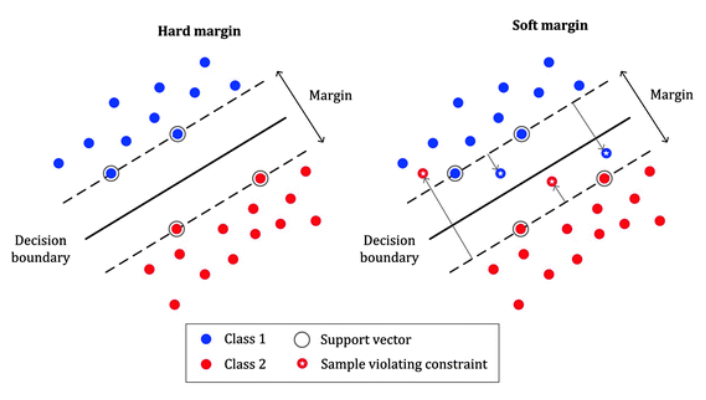
\includegraphics[width = 0.5\textwidth]{img/svm/margin.png}
    \caption{Hard margin vs. Soft margin}
    \label{fig:soft_margin}
\end{figure}
L'introduzione di questa variabile ci porta a modificare il problema di ottimizzazione
in questo modo:
\begin{equation}
    \begin{aligned}
        \min \left(\frac{1}{2} \| w \|^2 + C \cdot \sum_{i} \xi_i \right) \\
        \text{s.t.} \ y_i (\langle w, x_i \rangle + b) \geq 1 - \xi_i     \\
        \xi_i \geq 0
    \end{aligned}
\end{equation}
dove $C$ rappresenta il \textbf{complexity hyperparameter} e permette di
controllare la tolleranza  tra una classificazione errata e la larghezza del 
margine:
\begin{itemize}
    \item Se $C$ tende a infinito, allora si ha un hard margin.
    \item Se $C$ ha un valore grande si crea un hard margin che ammette pochi
          errori.
    \item Se $C$ ha un valore piccolo si crea un soft margin che ammette molti
          errori.
\end{itemize}
\section{Punti non sono linearmente separabili}
Quando si lavora con punti non linearmente separabili si usa lo stesso approccio,
rivedendo la formulazione del problema tramite i \textbf{metodi kernel}.
Si cerca di mappare lo spazio di input in un nuovo spazio, solitamente di
dimensione maggiore, in cui i punti siano linearmente separabili, in questo modo
è possibile classificare anche esempi non separabili linearmente.

Per effettuare questa trasformazione, dobbiamo trovare una funzione che prende
il nome di \textbf{funzione di trasformazione}:
\begin{equation}
    \Phi: \mathbb{R}^n \to \mathbb{R}^m, \ \text{con} \ m > n
\end{equation}
che mappi i dati iniziali non linearmente separabili in uno spazio di dimensione
superiore in cui siano linearmente separabili.

In questo nuovo spazio la funzione di decisione che classifica l'input $x$ è:
\begin{equation}
    sgn\left(\sum_{i \in Q} \alpha_i \cdot \langle \Phi(x_i), \Phi(x)\rangle + b
    \right)
\end{equation}
Il calcolo delle funzioni di trasformazione $\Phi$ è in generale computazionalmente
pesante, ma è semplificato nel caso di funzioni kernel.
\begin{definizione}[\textbf{Funzione kernel}]
    Data una trasformazione $\Phi: \mathbb{R}^n \to \mathbb{R}^m$ una
    \textbf{funzione kernel} è una mappa:
    \begin{equation}
        K: \mathbb{R}^n \times \mathbb{R}^n \to \mathbb{R} \ \text{tale che} \
        K(x, y) = \Phi(x) \cdot \Phi(y)
    \end{equation}
\end{definizione}
\begin{definizione}[\textbf{Kernel trick}]
    Si definisce quindi il \textbf{kernel trick} ovvero una procedura che permette
    di computare il prodotto interno delle trasformazioni dei due vettori $x$ e
    $y$, ovvero $\langle\Phi(x), \ \Phi(y)\rangle$, senza computare le
    trasformazioni. Questo permette di semplificare il calcolo di:
    \begin{equation}
        sgn\left(\sum_{i \in Q} \alpha_i \cdot \langle \Phi(x_i), \Phi(x) \rangle
        + b \right)
    \end{equation}
    sostituendo $\langle\Phi(x), \ \Phi(y)\rangle$ con $K(x_i, x)$, ottenendo:
    \begin{equation}
        sgn\left(\sum_{i \in Q} \alpha_i \cdot K(x_i, x) + b \right)
    \end{equation}
\end{definizione}
\begin{nota}
    Non si cercano tutte le possibili trasformazioni ma solo alcune.
\end{nota}
\begin{esempio}
    Sia $\Phi:\mathbb{R}^2\rightarrow\mathbb{R}^3$ la funzione di trasformazione
    definita nel seguente modo:
    \begin{equation}
        \Phi(x,y) =(x^2,y^2,\sqrt{2xy})
    \end{equation}
    avremo che $p_1 = (x_1, y_1), p_2 = (x_2, y_2) \in \mathbb{R}^2$, allora ho
    $K(p_1, p_2) = \langle \Phi(p_1), \Phi(p_2) \rangle \in\mathbb{R}^3$,
    più precisamente:
    $$K(p_1,p_2) = \left\langle\left(\begin{array}{c}
                x_1^2 \\
                y_1^2 \\
                \sqrt{2x_1y_1}
            \end{array}\right),\left(\begin{array}{c}
                x_2^2 \\
                y_2^2 \\
                \sqrt{2x_2y_2}
            \end{array}\right)\right\rangle = (x_1 \cdot x_2)^2 + (y_1 \cdot
        y_2)^2 + 2 \sqrt{x_1 \cdot y_1 \cdot x_2 \cdot y_2}$$
\end{esempio}
Si hanno alcune proprietà:
\begin{itemize}
    \item Se i dati sono mappati in uno spazio di dimensioni sufficientemente
          elevate, saranno quasi sempre linearmente separabili.
    \item Quattro dimensioni sono sufficienti per separare linearmente un cerchio
          in qualsiasi punto del piano.
    \item Cinque dimensioni sono sufficienti per separare linearmente qualsiasi
          ellisse.
    \item Se abbiamo $N$ esempi sono sempre separabili in spazi di dimensioni
          $N - 1$ o più.
    \item Calcolare $K(x, y)$ può essere molto economico anche se $\Phi(x)$ è
          molto costoso, ad esempio con vettori di dimensione elevata e, in tali
          casi (che vanno dimostrati), si addestrano le SVM nello spazio di
          dimensionalità maggiore senza mai dover trovare o rappresentare
          esplicitamente i vettori $\Phi(x)$.
\end{itemize}
Vediamo una lista di kernel standard:
\begin{itemize}
    \item \textbf{Lineare}: $K(x, y) = x \cdot y$
    \item \textbf{Polinomiale}: $K(x, y) = (1 + x \cdot y)^d$
    \item \textbf{Radial basis function}: $K(x, y) = e^{-\gamma \| x - y\|^2}$
    \item \textbf{Gaussian radial basis function}: $K(x, y) = e^{\frac{-(x-y)^2}
                      {2 \cdot \sigma^2}}$
    \item \textbf{Percettrone multistrato}: $K(x, y) = \tanh(b(x \cdot y) - c)$
\end{itemize}
\begin{teorema}
    Un kernel definisce una matrice $K_{i,j}$ che è simmetrica e definita positiva.
\end{teorema}
\begin{teorema}[\textbf{Teorema di Mercer}]
    Ogni matrice simmetrica e definita positiva è un kernel.
\end{teorema}
\begin{definizione}[\textbf{Gram matrix}]
    Definiamo \textbf{kernel matrix}, detta anche \textbf{matrice di Gram},
    dato un kernel $K$ e un insieme di punti $x_1, \dots, x_n$ come una matrice
    dove ogni componente è:
    \begin{equation}
        G_{i, j} = \langle \Phi(x_i), \Phi(x_j) \rangle = K(x_i, x_j)
    \end{equation}
\end{definizione}
\begin{esempio}
    Considerando il seguente dataset:
    \begin{equation}
        x_1 = [1, 2], \ x_2 = [3, 4], \ x_3 = [5, 6]
    \end{equation}
    dove a ogni istanza è associata la rispettiva classe:
    \begin{equation}
        y_1 = 1, \ y_2 = -1, \ y_3 = 1
    \end{equation}
    e il seguente kernel:
    \begin{equation}
        K(x, y) = x^T \cdot y
    \end{equation}
    si vuole calcolare la matrice di Gram per il kernel $K$ usando il dataset.
    Dalla definizione della matrice di Gram si ha che:
    \begin{equation}
        G = \left[
            \begin{array}{ccc}
                K(x_1, x_1) & K(x_1, x_2) & K(x_1, x_3) \\
                K(x_2, x_1) & K(x_2, x_2) & K(x_2, x_3) \\
                K(x_3, x_1) & K(x_3, x_2) & K(x_3, x_3) \\
            \end{array}
            \right] = \left[
            \begin{array}{ccc}
                1 \cdot 1 + 2 \cdot 2 & 1 \cdot 3 + 2 \cdot 4 & 1 \cdot 5 + 2 \cdot 6 \\
                3 \cdot 1 + 4 \cdot 2 & 3 \cdot 3 + 4 \cdot 4 & 3 \cdot 5 + 4 \cdot 6 \\
                5 \cdot 1 + 6 \cdot 2 & 5 \cdot 3 + 6 \cdot 4 & 5 \cdot 5 + 6 \cdot 6 \\
            \end{array}
            \right] = \left[
            \begin{array}{ccc}
                5  & 11 & 17 \\
                11 & 25 & 39 \\
                17 & 39 & 61 \\
            \end{array}
            \right]
    \end{equation}
\end{esempio}
\section{Classificazione multi-classe}
SVM può essere applicato a problemi non binari tramite \textit{one vs rest},
ovvero consiste nell'effettuare, per ogni classe, un'esecuzione di SVM tra la singola classe
contro tutte le altre. In aggiunta, si combinano tutti gli iperpiani trovati
tra di loro per effettuare la classificazione multi-classe.

Si ha quindi l'addestramento di un singolo classificatore per classe, con i campioni
di quella classe considerati come positivi e tutti gli altri campioni come negativi.

Questa strategia richiede che i classificatori di base producano un punteggio di
confidenza a valore reale per la sua decisione, piuttosto che solo un'etichetta
di classe; infatti, le sole etichette di classi discrete possono portare a ambiguità.
Abbiamo quindi:
\begin{itemize}
    \item Come input:
          \begin{itemize}
              \item Un learner $L$
              \item Un set di esempi $X$
              \item Delle label $y_i$ associate ad ogni $x_i \in X$ con $i = 1, \dots, K$
          \end{itemize}
    \item Come output una lista di classificatori $f_k$ con $k = 1,\dots, K$
\end{itemize}
La procedura di training consiste nel generare per ogni istanza $x_i$ un vettore 
di label $z_i$ di $k$ componenti, una per ogni classe, definito in questo modo:
\begin{equation}
    z_i = \begin{cases}
        y_i & \text{se} \ x_i \in \text{classe}(k) \\
        0   & \text{altrimenti}
    \end{cases}
\end{equation}
Quindi l'input per la fase di training del learner $L$ diventa $(x_i,z_i)$ e l'algoritmo
consiste nell'eseguire i singoli $k$ learner su $x_i$, i quali calcoleranno
$p_{ik}$ che sarà la componente del vettore di predizione delle label $p_i$ associata
alla classificazione della classe $k$. Successivamente si confronterà $z_i$ e $p_i$
per vedere se sono stati classificati correttamente gli esempi.

Quindi prendere decisioni significa applicare tutti i classificatori ad un nuovo
esempio e prevedere l'etichetta $k$ per la quale il classificatore corrispondente
riporta il punteggio di confidenza più alto:
\begin{equation}
    \hat{y} = argmax f_k(x), \ k \in \{1,\dots K\}
\end{equation}
Questa euristica soffre di diversi problemi:
\begin{itemize}
    \item La scala dei valori di confidenza può differire tra vari classificatori
          binari
    \item Anche se la distribuzione in classe è bilanciata nel training set, i
          learner per la classificazione binaria vedono distribuzioni sbilanciate
          perché tipicamente l'insieme di negativi che vedono è molto più grande
          dell'insieme di positivi.
\end{itemize}
Un'alternativa è \textit{one vs one} prendendo le varie classi e produrre sistemi
di SVM tra coppe di classe. La quantità di problemi derivati esplode in modo
quadratico. Alla fine, si attribuisce maggior probabilità ad una singola classe.
Si ha il train di:
\begin{equation}
    \frac{K \cdot (K - 1)}{2}
\end{equation}
classificatori binari per un problema a $K$ classi e ognuno riceve i campioni di
un paio di classi dal training set originale e deve imparare a distinguere queste
due classi.

In fase di predizione tutti i $\frac{K \cdot (K - 1)}{2}$ classificatori sono
applicati al nuovo sample e la classe che con il più alto numero di predizioni
positive viene usata come previsione per il classificatore combinato. Anche
questa tecnica soffre di ambiguità in quanto alcune regioni del suo spazio di
input possono ricevere lo stesso numero di voti.